\chapter{Устойчивость}

\section{Линейная устойчивость стационарных мод}	

Как упоминалось ранее, важной характеристикой стационарного решения является его устойчивость.
Зачастую, лишь устойчивые стационарные моды можно получить в реальном физическом эксперименте.
В этой главе рассматривается устойчивость локализованных стационарных состояний уравнения (\ref{eq:initial}) в случае простейшей нелинейной периодической модуляции $U(x) \equiv 0$, $P(x) = \alpha + \cos 2x$.
Уравнение (\ref{eq:initial}) принимает вид
%
\begin{equation}
i\Psi_t + \Psi_{xx} + (\alpha + \cos 2x) |\Psi|^2 \Psi = 0.
\label{eq:stability}
\end{equation}
%

Ранее в Главе 2 было показано, что класс стационарных локализованных решений уравнения (\ref{eq:stability}) чрезвычайно широк.
Следуя общепринятому подходу к исследованию линейной устойчивости \cite{JYang}, рассмотрим малые возмущения стационарного решений $\Psi_0(x,t) = u(x)e^{- \omega t}$ в виде:
%
\begin{equation}
\Psi(x,t) = \left[ u(x) +  \widetilde{U}(x,t) \right] e^{-i \omega t}, \quad \left|\widetilde{U}(x,t) \right| \ll 1,
\label{eq:perturbation}
\end{equation}
%
где $u(x)$ --- локализованное решение уравнения (\ref{eq:stationary_obj}), а $\widetilde{U}(x,t)$ --- малая комплекснозначная функция-возмущение.
Подставляя $\Psi(x,t)$ в эволюционное уравнение (\ref{eq:stability}) и линеаризуя получившееся соотношение относительно $\widetilde{U}(x,t)$, получаем
%
\begin{equation}
i \widetilde{U}_t + \widetilde{U}_{xx} + \omega \widetilde{U} + (\alpha + \cos 2x)u^2 (2 \widetilde{U} + \widetilde{U}^*) = 0,
\label{eq:perturb_evolution}
\end{equation}
%
где звездочка $(^*)$ означает операцию комплексного сопряжения.
Будем искать решение уравнения (\ref{eq:perturb_evolution}) для возмущения в виде
%
\begin{equation}
\widetilde{U}(x,t) = (v(x) + w(x))e^{\lambda t} + (v^*(x) - w^*(x))e^{\lambda^* t}.
\label{eq:seeking}
\end{equation}
%
Получаем задачу на собственные значения дифференциального оператора
%
\begin{equation}
LY = \lambda Y
\label{eq:eigproblem}
\end{equation}
%
\begin{equation}
L = i \begin{pmatrix}
0 & L_0 \\
L_1 & 0
\end{pmatrix}, \quad
Y = \begin{pmatrix}
v \\
w
\end{pmatrix},
\label{eq:operators}
\end{equation}
%
где
%
\begin{eqnarray*}
&& L_0 = \partial_{xx} + G_0(x), \quad G_0(x) = \omega + (\alpha + \cos 2x) u^2; \\
&& L_1 = \partial_{xx} + G_1(x), \quad G_1(x) = \omega + 3(\alpha + \cos 2x) u^2.
\end{eqnarray*}
%
Спектр дифференциального оператора (\ref{eq:eigproblem}) определяет линейную устойчивость стационарной моды.
Стационарное решение является линейно неустойчивым, если спектр соответствующего оператора содержит хотя бы одно собственное значение $\lambda$ с ненулевой действительной частью $\Re(\lambda) > 0$.
В противном случае решение будет линейной устойчивым.

Спектр оператора (\ref{eq:eigproblem}) состоит из двух частей: непрерывный и дискретный спектры.
Непрерывный спектр можно получить в пределе при $|x| \to \infty$, когда $u(x)$ стремиться к нулю, поскольку является локализованным решением.
В этом случае операторы $L_0$, $L_1$ линеаризуются и принимают вид $\partial_{xx} + \omega$, и $L$ становится обыкновенным дифференциальным оператором с постоянными коэффициентами.
Решая соответствующее дифференциальное уравнение несложно показать, что непрерывный спектр представляет собой два луча, $[-i \omega; +i \infty)$ и $( -i \infty; i \omega]$, в случае $\omega < 0$ и заполняет всю мнимую ось, кода $\omega > 0$.
Нулевое собственное значение принадлежит дискретному спектру.
Остальные собственные значения в дискретном спектре появляются парами или четверками в силу симметрии уравнения (\ref{eq:eigproblem}), заключающееся в том, что если $\lambda$ является собственным значением, то $-\lambda$, $\pm \lambda^*$ также являются собственными значениями оператора (\ref{eq:eigproblem}).

Поиск дискретного спектра мы осуществим численно с помощью так называемого метода коллокаций Фурье (Fourier collocation method, FCM) \cite{JYang}.
Для начала будем считать, что нелинейная мода локализована на промежутке длины $L$, и от рассмотрения моды на всей действительной оси, мы перейдем к ее рассмотрению на конечном интервале $[-L/2; L/2]$.
На этом интервале представим собственную функцию $Y = (v(x), w(x))^T$, а также функции $G_0$, $G_1$ в виде рядов Фурье
%
\begin{eqnarray}
&& v(x) = \sum \limits_n a_n e^{i n k_0 x}, \quad w(x) = \sum \limits_n b_n e^{i n k_0 x}, \\
&& G_j(x) = \sum \limits_n c_n^{(j)} e^{i n k_0 x}, \quad j = 0, 1,
\end{eqnarray}
%
где $k_0 = 2 \pi / L$.
Поставляя эти разложения в уравнения (\ref{eq:eigproblem}), получим новую задача на собственные значения c неизвестными коэффициентами $a_j$, $b_j$ вида
%
\begin{eqnarray}
&& -(k_0 j)^2 b_j + \sum \limits_n c_n^{(0)} b_{j-n} = -i \lambda a_j; \\
&& -(k_0 j)^2 a_j + \sum \limits_n c_n^{(1)} a_{j-n} = -i \lambda b_j,
\end{eqnarray}
%
где $-\infty < j < +\infty$.
Будем считать, что первые $N$ гармоник соответствующих рядом Фурье достаточно хорошо описывают нелинейную моду, что позволяет перейти от рассмотрения бесконечного числа гармоник к конечному их числу $-N \le j \le +N$.
Получаем задачу на собственные значения для обыкновенного конечного линейного оператора
%
\begin{equation}
i \begin{pmatrix}
0 & D + C_0 \\
D + C_1 & 0
\end{pmatrix}
\begin{pmatrix}
A \\ B
\end{pmatrix}
= \lambda
\begin{pmatrix}
A \\ B
\end{pmatrix}.
\label{eq:eigproblem_alg}
\end{equation}
%
Здесь
%
\begin{eqnarray}
&& A = (a_{-N}, a_{-N+1}, \dots, a_N)^T, \\
&& B = (b_{-N}, b_{-N+1}, \dots, b_N)^T, \\
&& D = (i k_0)^2 \diag(-N, -N+1, \dots, N)^2, 
\end{eqnarray}
%
а матрицы $C_j$, $j = 1,2$ имеют вид
%
\begin{equation}
C_j = 
\begin{pmatrix}
c_0^{(j)} & c_{-1}^{(j)} & \dots & c_{-N}^{(j)} & 0 & 0 & \dots & 0 \\
c_1^{(j)} & c_0^{(j)} & c_{-1}^{(j)} & \dots & c_{-N}^{(j)} & 0 & \dots & 0 \\
\vdots & \vdots & \vdots & \ddots & \vdots & \vdots & \vdots & \vdots \\
0 &\dots & 0 & 0 & c_N^{(j)} & \dots & c_1^{(j)} & c_0^{(j)}
\end{pmatrix}
\end{equation}
%
Далее задача (\ref{eq:eigproblem_alg}) на собственные значения решалась численно с помощью QR-алгоритма.

Заметим, что такой метод хорошо подходит для определения {\it экспоненциальной неустойчивости}, появляющейся вследствие наличия действительных  собственных значений.
Однако известно, что это метод может подвести в случае {\it осцилляторной неустойчивости}, вызванной четверками комплексных собственных значений с малыми действительными частями \cite{Kizin}.
В таких случаях необходимо проводить более тонкие исследования другими методами, например, используя аппарат функции Эванса \cite{Pelinovsky}.

Используя FCM было проанализировано большое количество стационарных нелинейных решений уравнения (\ref{eq:stationary_obj}), которым соответствовали различные коды.
В связи с бесконечным количеством разнообразных стационарных решений, невозможно выполнить анализ линейной устойчивости всех стационарных мод, даже в случае элементарных солитонов.
Однако в ходе многочисленных экспериментов наметилась общая тенденция, что практически все локализованные стационарные моды уравнения (\ref{eq:stationary_obj}) оказываются линейно неустойчивыми.

Что касается устойчивых образований, то было обнаружено, что фундаментальный солитон (FS), Рис. \ref{pic:stability}, (A), его код $\{ \dots, O, A_{\pm 1}, O, \dots \}$ и дипольный солитон (DS), Рис. \ref{pic:stability} (G), $\{ \dots, O, B_{\pm 1}, O, \dots \}$, линейно устойчивы при некоторых ограничениях на параметры $\omega$, $\alpha$.
Результаты, относящиеся к устойчивости FS, согласуются с теми, что были получены в работе \cite{Malomed}.
Остальные элементарные солитоны оказываются неустойчивыми.
Некоторые комплексы FS, к примеру, соответствующие кодам $\{ \dots, A_1, A_{-1}, A_1, O, \dots \}$, $\{ \dots, O, A_1, O, A_{-1}, O, \dots \}$, также оказываются устойчивыми.
Однако большая часть таких комплексов все же оказывается неустойчивой.
Некоторые примеры локализованных стационарных мод и спектры соответствующих им операторов для значений параметров $\omega = -1$, $\alpha = -0.2$ показаны на Рис. \ref{pic:stability}.
%
\begin{figure}
	\begin{minipage}[h]{0.5\linewidth}
	\center{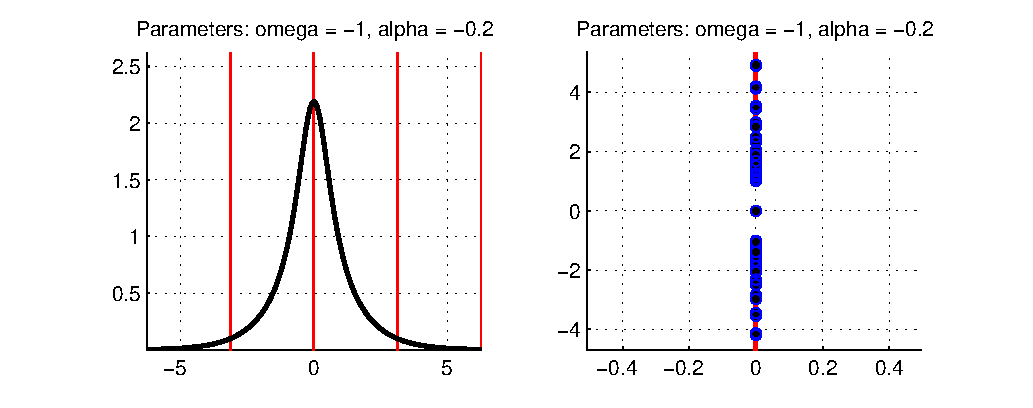
\includegraphics[width=1\linewidth]{pic/OA1O.eps} \ (A) $\{ \dots,O,A_1,O,\dots \}$}
	\end{minipage}
\hfill
	\begin{minipage}[h]{0.5\linewidth}
	\center{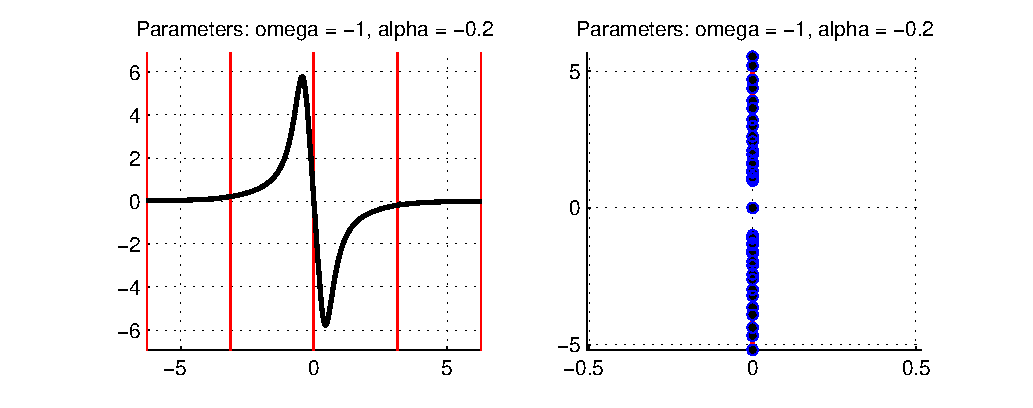
\includegraphics[width=1\linewidth]{pic/OB-1O.eps} \ (B) $\{ \dots,O,B_{-1},O,\dots \}$}
	\end{minipage}
\vfill
	\begin{minipage}[h]{0.5\linewidth}
	\center{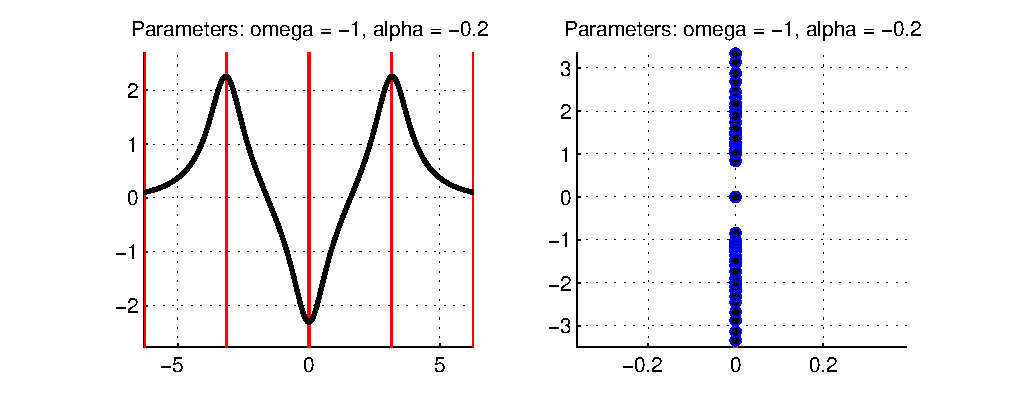
\includegraphics[width=1\linewidth]{pic/OA1A-1A1O.eps} \ (C) $\{ \dots,O,A_1,A_{-1},A_1,O,\dots \}$}
	\end{minipage}
\hfill
	\begin{minipage}[h]{0.5\linewidth}
	\center{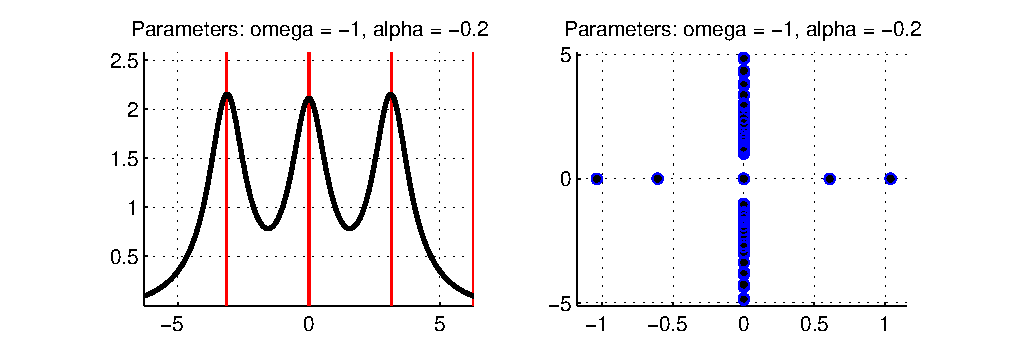
\includegraphics[width=1\linewidth]{pic/OA1A1A1O.eps} \ (D) $\{ \dots,O,A_1,A_1,A_1,O,\dots \}$}
	\end{minipage}
\vfill
	\begin{minipage}[h]{0.5\linewidth}
	\center{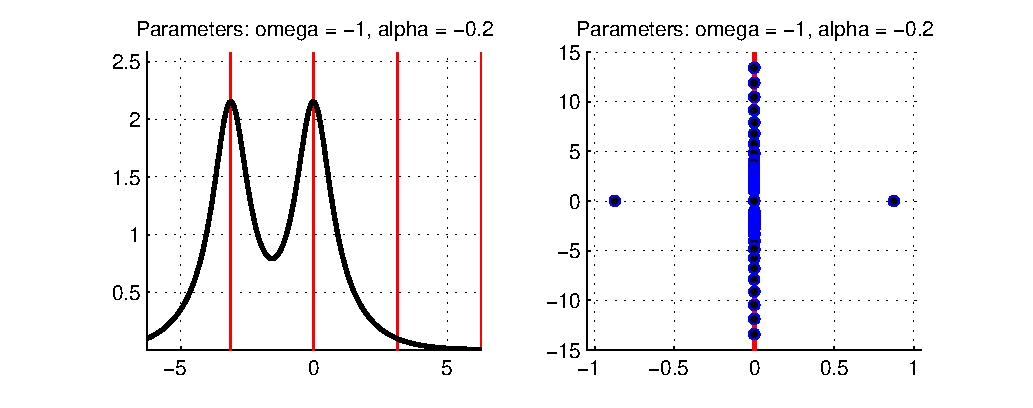
\includegraphics[width=1\linewidth]{pic/OA1A1O.eps} \ (E) $\{ \dots,O,A_1,A_1,O,\dots \}$}
	\end{minipage}
\hfill
	\begin{minipage}[h]{0.5\linewidth}
	\center{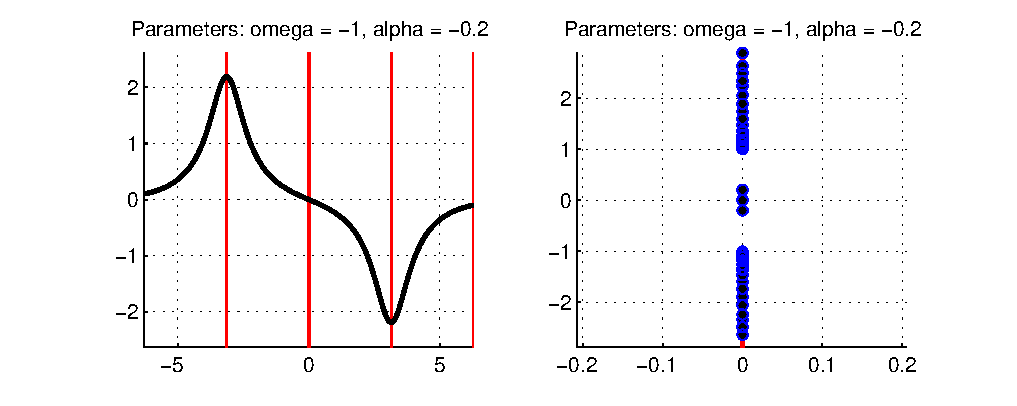
\includegraphics[width=1\linewidth]{pic/OA1OA-1O.eps} \ (F) $\{ \dots,O,A_1,O,A_{-1},O,\dots \}$}
	\end{minipage}
\vfill
	\begin{minipage}[h]{0.5\linewidth}
	\center{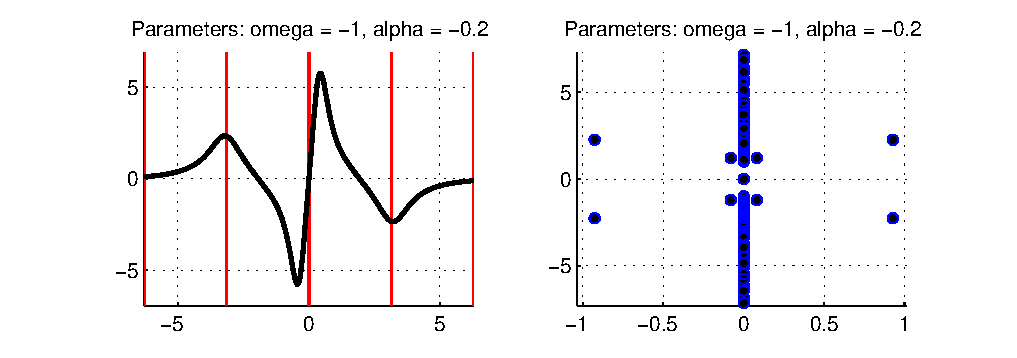
\includegraphics[width=1\linewidth]{pic/OA1B1A-1O.eps} \ (G) $\{ \dots,O,A_1,B_1,A_{-1},O,\dots \}$}
	\end{minipage}
\hfill
	\begin{minipage}[h]{0.5\linewidth}
	\center{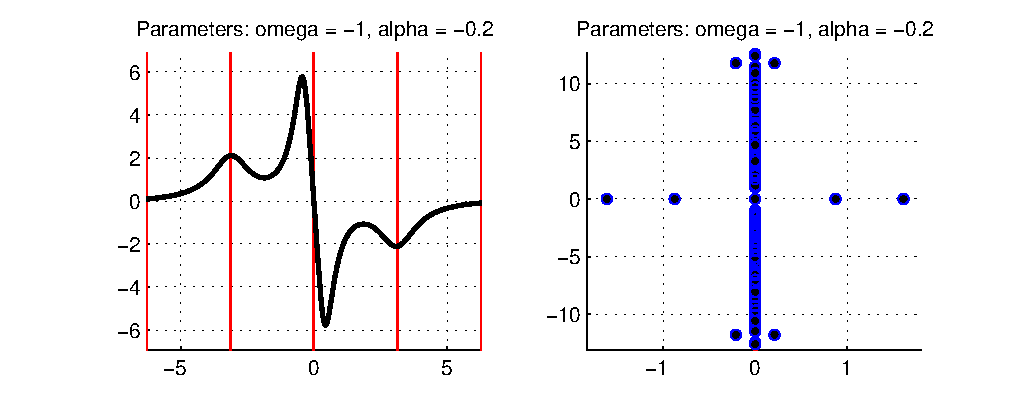
\includegraphics[width=1\linewidth]{pic/OA1B-1A-1O.eps} \ (H) $\{ \dots,O,A_1,B_{-1},A_{-1},O,\dots \}$}
	\end{minipage}
\caption{Локализованные решения, их коды и спектры линейной устойчивости соответствующих им операторов для значений параметров $\omega = -1$, $\alpha = -0.2$}
\label{pic:stability}
\end{figure}
%

Напомним, что в работе \cite{Malomed} была подробно исследована устойчивость FS решений как численно, так и аналитически, используя метод вариационной аппроксимации.
Существование в задаче (\ref{eq:stationary_obj}) устойчивого класса DS решений ранее не было известно и не обсуждалось в литературе.
Поэтому далее в этой главе мы подробно рассмотрим вопрос устойчивости дипольного солитона.

\section{DS: вариационная аппроксимация}

Некоторые общие свойства солитонных решений уравнения (\ref{eq:stationary_obj}) можно получить методом {\it вариационной аппроксимации} (ВА), принимая во внимание тот факт, что уравнение для стационарных состояний может быть получено из соответствующего лагранжиана
%
\begin{equation}
L = \int \limits_{-\infty}^{+\infty} \Big\{ \dfrac{1}{2} (u')^2 - \dfrac{1}{2} \omega u^2 - \dfrac{1}{4} [\alpha + \cos 2x] u^4 \Big\}.
\label{eq:lagrangian}
\end{equation}
%
В работе \cite{Malomed}, ВА была применена для анализа FS решений.
Для этого использовалась следующая подстановка:
%
\begin{equation}
u(x) = A \exp \left( -\dfrac{x^2}{2 W^2} \right),
\label{ea:fs_ansatz}
\end{equation}
%
отражающая тот факт, что FS решения имеют колоколообразную форму. 
В результате применения этого подхода, был предсказан факт наличия минимальной нормы FS решения
%
\begin{equation}
N \equiv \int \limits_{-\infty}^{+\infty} u^2(x) dx = \sqrt{\pi} A^2 W,
\end{equation}
%
а также существование порога устойчивости по амплитуде.

Аналогичное исследование для дипольного солитона (DS) произведем с помощью простейшей нечетной локализованной подстановки:
%
\begin{equation}
u(x) = Ax \exp \left( -\dfrac{x^2}{2 W^2} \right).
\label{eq:ds_ansatz}
\end{equation}
%
Максимальное значение $u(x)$, равное $\sqrt{e}AW$, достигается в $x_{max} = W$.
Следовательно параметр $W$ имеет значение полуширины дипольного солитона.
Норма соответствующей подстановки (\ref{eq:ds_ansatz}) равна
%
\begin{equation}
N = \dfrac{\sqrt{\pi}}{2} A^2 W^3.
\label{ds_norm}
\end{equation}
%
Уравнение (\ref{ds_norm}) позволяет выразить амплитуду через норму:
%
\begin{equation}
A^2 = \dfrac{2}{\sqrt{\pi}} \dfrac{N}{W^3}.
\label{eq:amplitude}
\end{equation}
% 
Подставляя соотношения (\ref{eq:ds_ansatz}), (\ref{eq:amplitude}) в лагранжиан (\ref{eq:lagrangian}) и, далее, интегрируя получившееся выражение, получаем следующее выражение для эффективного лагранжиана:
%
\begin{equation}
L_{\mathrm{eff}}=-\frac{\omega }{2}N+\frac{3N}{4W^{2}}-\frac{3\alpha N^{2}}{16\sqrt{2\pi}W}-\frac{N^{2}e^{-W^{2}/2}}{16\sqrt{2\pi}W}\left(3-6W^{2}+W^{4}\right).
\label{eq:lagrangian_eff}
\end{equation}
%
Вариационные уравнения Эйлера-Лагранжа для эффективного лагранжиана (\ref{eq:lagrangian_eff}) имеют вид
%
\begin{eqnarray}
\partial L_{\mathrm{eff}}/\partial W = 0; \label{eq:dw} \\
\partial L_{\mathrm{eff}}/\partial N = 0, \label{eq:dn}
\end{eqnarray}
%
где $W$ и $N$ --- свободные вариационные параметры для заданного $\omega$.

Далее, вслед за авторами работы \cite{Malomed}, рассматривается случай $\alpha = 0$.
Уравнение (\ref{eq:dw}) позволяет получить связь величин $N$ и $W$ вида:
%
\begin{equation}
N=\frac{48\sqrt{\pi /2}\exp \left( W^{2}/2\right) }{W\left(3+9W^{2}-9W^{4}+W^{6}\right) }.
\label{eq:N(W)}
\end{equation}
%
Это соотношение изображено на Рис. \ref{pic:N(W)}.
%
\begin{figure}
\center{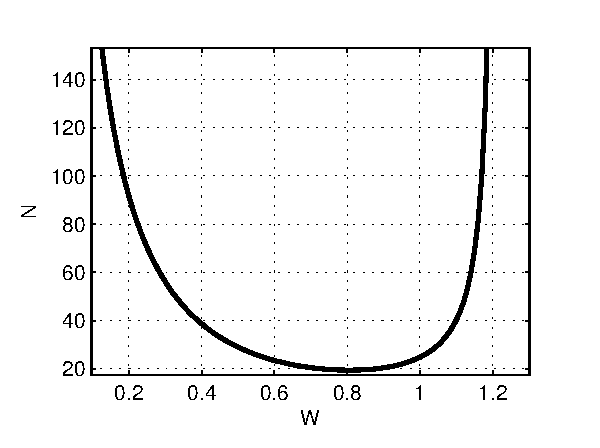
\includegraphics[width=0.5\textwidth]{pic/N(W).eps}}
\caption{Соотношение между нормой и полушириной дипольного солитона, предсказываемое вариационной аппроксимацией, $\alpha = 0$}
\label{pic:N(W)}
\end{figure}
%
Минимальное значение нормы дипольного солитона, предсказываемое вариационной аппроксимацией, достигается при значении $W = W_0 \approx 0.806$ и равно
%
\begin{equation}
N_{\mathrm{min}}^{\mathrm{(VA)}} \approx 19.41
\label{eq:norm_min_va}
\end{equation}
%

Таким образом, вариационная аппроксимация предсказывает существование минимальной нормы, при которой существует дипольный солитон.
В терминах БЭК это означает, что дипольный солитон не наблюдается при малом количестве частиц, образующих конденсат.
Более того, из соотношения (\ref{eq:N(W)}) следует, что величина $W$ может изменять лишь в конечных пределах:
%
\begin{equation}
0 < W < W_{\mathrm{max}} \approx 1.21.
\end{equation}
%

Второе вариационное уравнений (\ref{eq:dn}) после некоторых преобразований обнаруживает монотонную зависимость между $\omega$ и $W$ вида
%
\begin{equation}
\omega =\frac{3}{2}\frac{-9+33W^{2}-13W^{4}+W^{6}}{W^{2}\left( 3+9W^{2}-9W^{4}+W^{6}\right) }.
\label{eq:omega}
\end{equation}
%
Объединяя это с соотношением (\ref{eq:N(W)}), применим критерий устойчивости Вахитова-Колоколова \cite{JYang}; $dN / d\omega \equiv (d\omega / dW)^{-1} dN / dW < 0$.
Из выражения (\ref{eq:omega}) следует, что величина $d\omega / dW$ всегда положительна.
Критерий Вахитова-Колоколова предсказывает устойчивость левой ветки решений типа DS на Рис. \ref{pic:N(W)}, где $dN / dW < 0$, что соответствует интервалу значений $W$
%
\begin{equation}
0 < W < W_0 \approx 0.806,
\end{equation}
%
в то время как правая ветка, $dN / dW > 0$, т.е. $W > W_0$ оказывается неустойчивой.
Стоит отметить, что сам метод вариационной аппроксимации дает крайне приближенные значение количественных характеристик в силу неточности метода, однако качественные предсказания оказываются весьма полезными.
Подведем итоги применения вариационной аппроксимации к классу решений типа DS.
Вариационная аппроксимация предсказывает, что
%
\begin{itemize}
\item[(a)] существует минимальная норма дипольного солитона;
\item[(б)] существует максимально возможная ширина дипольного солитона;
\item[(в)] существует граница по ширине DS, которая отделяет устойчивую ветку решений от неустойчивой.
\end{itemize}
%
В следующих разделах мы покажем, что все эти предсказания качественно согласуются с результатами численного эксперимента.

\section{DS: численное исследование}

Численное исследование семейства DS решений производилось численно с помощью метода стрельбы.
В этом разделе представлены основные результаты этого исследования.

Семейство DS решений может быть запараметризовано с помощью $\omega$ или же с помощью параметра $W$, который в нашем случае определен как расстояние от центральной точки до точки максимума DS солитона и имеет смысл полуширины дипольного солитона.
Было обнаружено, что амплитуда и норма растут при уменьшении характерной ширины солитона, т.е. когда $W$ стремиться к нулю, а $\omega$ стремиться к $-\infty$.
Примеры различных профилей изображены на Рис. \ref{pic:dss}
%
\begin{figure}
\center{\includegraphics[width=0.5\textwidth]{pic/DSs.eps}}
\caption{Численно построенные профили дипольных солитонов при значениях $\omega = -15$ (тонкая линия), $\omega = -7$ (пунктирная линия) и $\omega = -1$ (толстая линия) для $\alpha = 0$}
\label{pic:dss}
\end{figure}
%

Численно определенное соотношение нормы $N$ и полуширины $W$ изображено на Рис. \ref{pic:N(W)_numerical}.
Из этого графика видно, что существует минимальная норма, необходимая для существования дипольного солитона, как это и было предсказано с помощью вариационной аппроксимации (пункт (а)).
%
\begin{figure}
\center{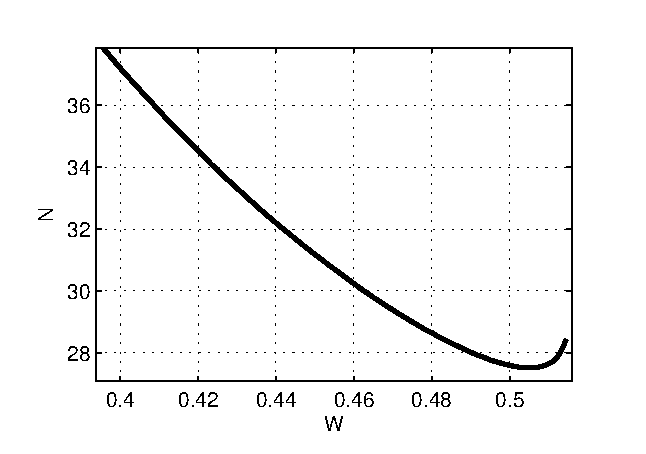
\includegraphics[width=0.5\textwidth]{pic/N(W)_numerical.eps}}
\caption{Численно построенная зависимость $N(W)$, нормы от полуширины дипольного солитона для $\alpha = 0$}
\label{pic:N(W)_numerical}
\end{figure}
%

С помощью численного счета было показано, что дипольный солитон, имеющий код $\{ \dots, O, B_{\pm 1}, O, \dots \}$, существует при $\omega < \omega^*$, где $\omega^* = 0.2654$.
В точке $\omega^*$ он претерпевает бифуркацию типа седло-узел и пропадает вместе с веткой решения, отвечающей коду $\{ \dots, O, A_{\mp 1}, B_{\pm 1}, A_{\pm 1}, O, \dots \}$.
Соответствующая бифуркационная диаграмма изображена на Рис. \ref{pic:bifurcation}.
Это означает, что ширина (полуширина $W$) ограничена сверху, как это и предсказывалось вариационной аппроксимацией (пункт (б)).

Таким образом результаты вариационной аппроксимации качественно согласуются с численным счетом, хотя точность такой аппроксимации недостаточна.
Например, минимальная норма, предсказанная с помощью ВА, оказывается на $30\%$ меньше численно полученного значения $N_{\mathrm{min}}^{\mathrm{(num)}} \approx 27.5$.
%
\begin{figure}
\center{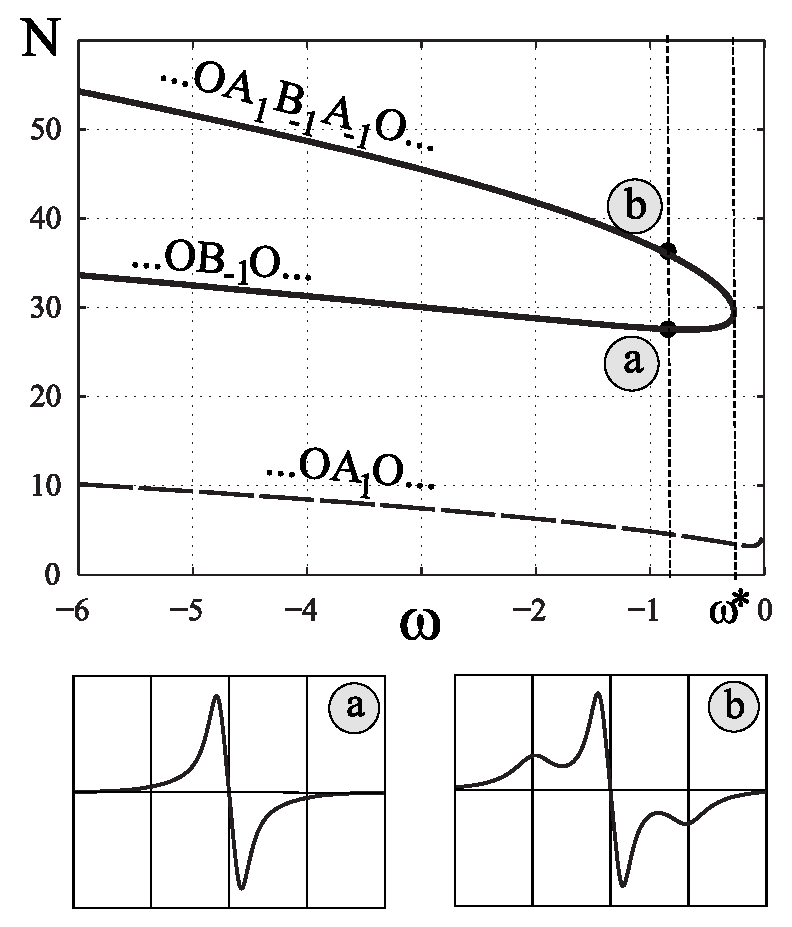
\includegraphics[width=0.5\textwidth]{pic/bifurcation.eps}}
\caption{Бифуркационная диаграмма при $\alpha = 0$: ветка решения типа DS, отвечающая коду $\{ \dots, O, B_{\pm 1}, O, \dots \}$ претерпевает бифуркацию и пропадает вместе с веткой решения, отвечающей коду $\{ \dots, O, A_{\mp 1}, B_{\pm 1}, A_{\pm 1}, O, \dots \}$. Два профиля соответствующих решений построены для значения $\omega = -0.8$.}
\label{pic:bifurcation}
\end{figure}
%

\section{DS: эволюционное моделирование}

С целью проверки предположения (в), полученного в результате применения вариационной аппроксимации, было произведено моделирование эволюции дипольного солитона во времени.
Для этого была использована консервативная конечно-разностная схема Трофимова-Пескова \cite{Trofimov}.
Эта схема замечательна тем, что сохраняет норму решения (\ref{eq:norm}) и значение функционала энергии (\ref{eq:energy}).
Она является неявной, однако позволяет проводить расчеты с большим временным шагом.
Для устранения эффекта отражения от концов был использован прием искусственной диссипации на краях.
С целью выявления неустойчивости стационарной моды, она возмущалась некоторым малым пространственным возмущением.
В расчетах использовалась конечная пространственная область $[-4\pi, 4\pi]$.

Некоторые результаты моделирования представлены на Рис. \ref{pic:evolution_unst}, \ref{pic:evolution_st}.
В случае, когда дипольный солитон оказывается неустойчивым, он перестраивается в устойчивый фундаментальный солитон.
Этот факт отражен на Рис. \ref{pic:evolution_unst} и Рис. \ref{pic:summary}.
Численный эксперимент позволяет заключить, что предсказание (в), полученное в результате вариационной аппроксимации, также верно.
Результаты моделирования удобно изобразить на графике $N(\omega)$, Рис. \ref{pic:summary}.
Левая ветка решения, где наклон графика $N(\omega)$ отрицателен, демонстрирует устойчивое поведение, в то время как правая ветка (наклон графика $N(\omega)$ положителен) неустойчива.
Этот факт согласуется с результатами вариационной аппроксимации и критерием Вахитова-Колоколова.
Однако точная граница между устойчивой и неустойчивой областью осталась неясна.
Это связано с тем, что для параметров $\omega$ вблизи минимума графика $N(\omega)$ эволюция дипольного солитона зависит от типа возмущения и параметров численного счета.
%
\begin{figure}
	\center{\begin{minipage}[h]{0.75\linewidth}
	\center{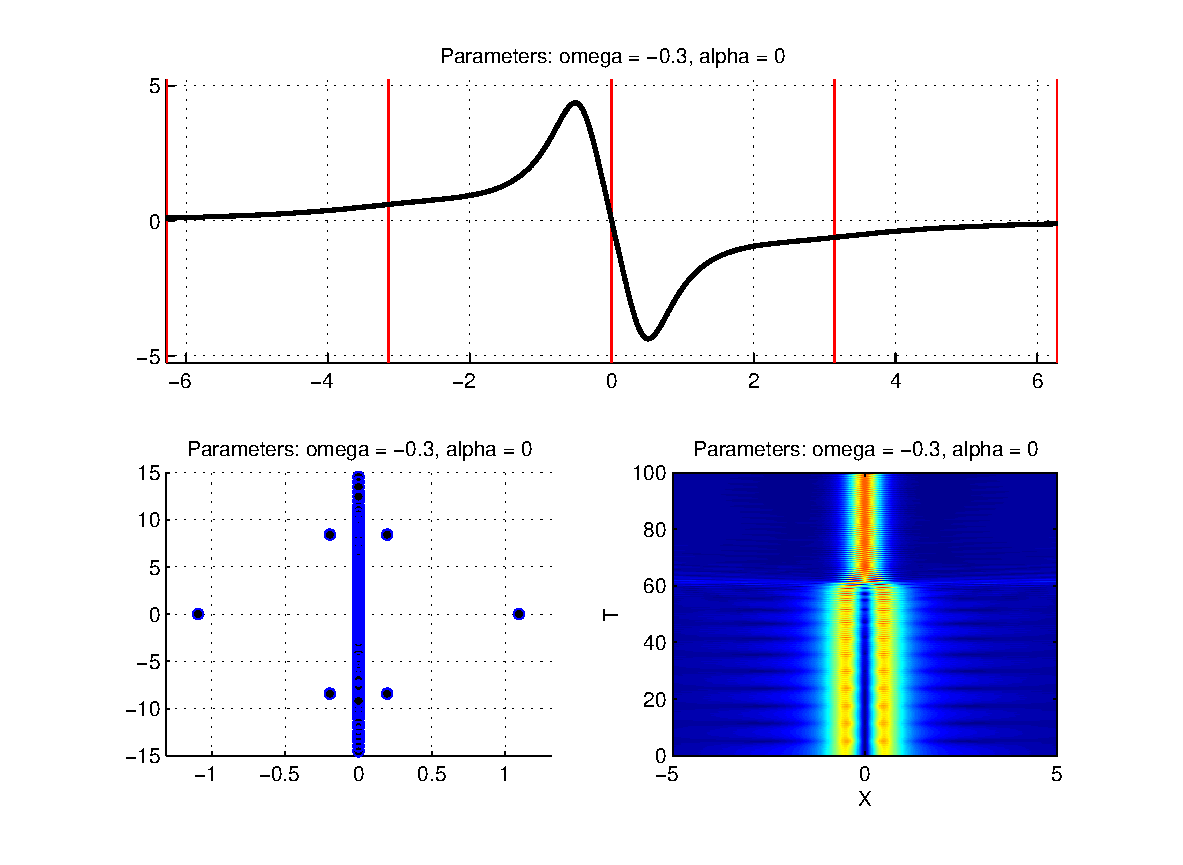
\includegraphics[width=1\linewidth]{pic/omega=-03alpha=0.eps} \ (A) $\omega = -0.3$}
	\end{minipage}}
	\center{\begin{minipage}[h]{0.75\linewidth}
	\center{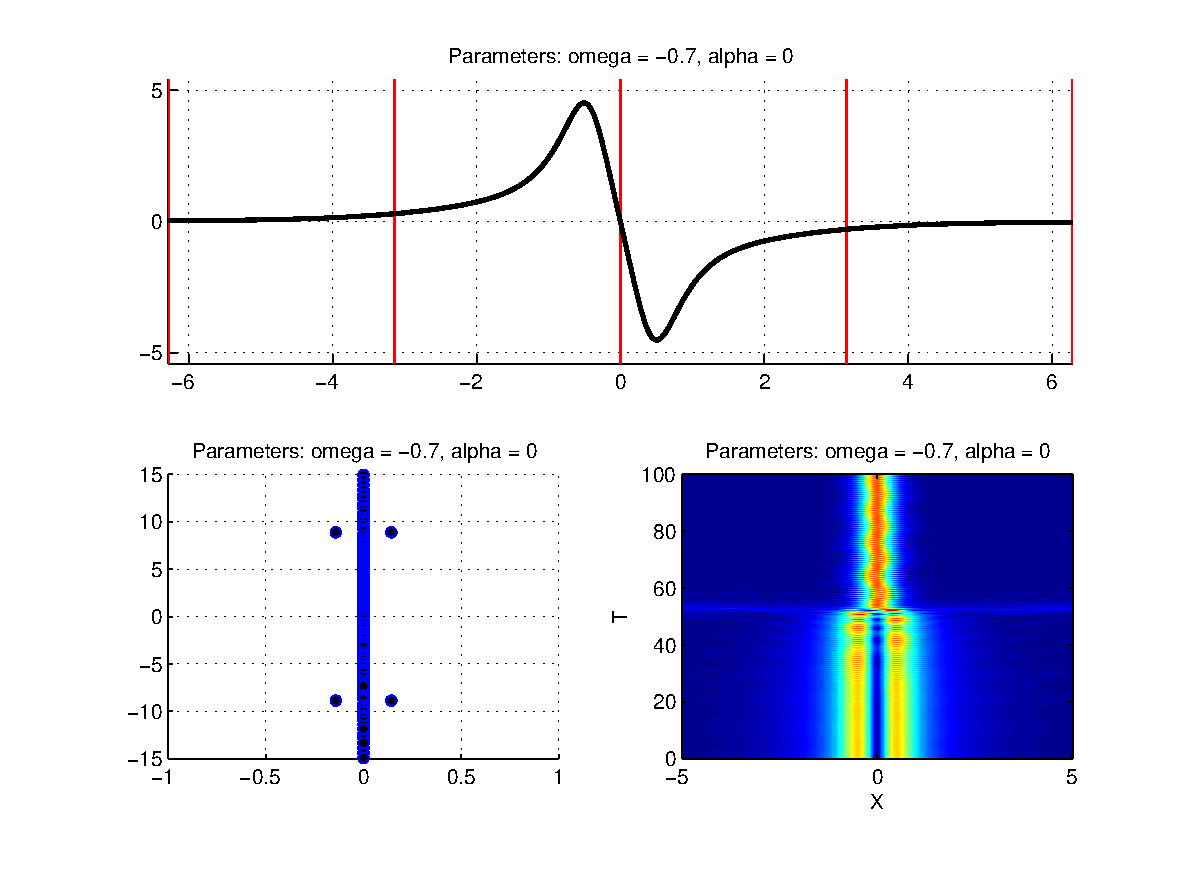
\includegraphics[width=1\linewidth]{pic/omega=-07alpha=0.eps} \ (B) $\omega = -0.7$}
	\end{minipage}}
\caption{Эволюция неустойчивых дипольных солитонов и соответствующие им спектры при $\alpha = 0$.}
\label{pic:evolution_unst}
\end{figure}
%
\begin{figure}
	\center{\begin{minipage}[h]{0.75\linewidth}
	\center{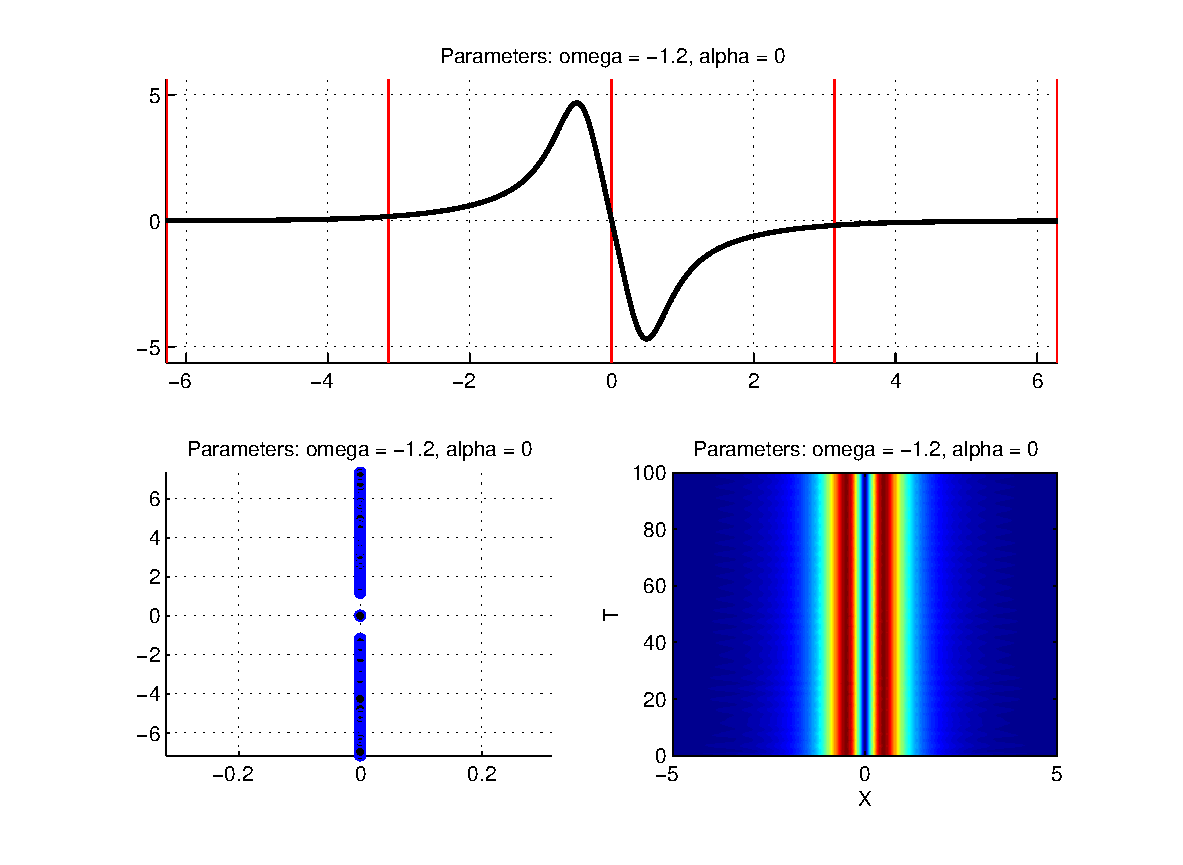
\includegraphics[width=1\linewidth]{pic/omega=-12alpha=0.eps} \ (A) $\omega = -1.2$}
	\end{minipage}}
	\center{\begin{minipage}[h]{0.75\linewidth}
	\center{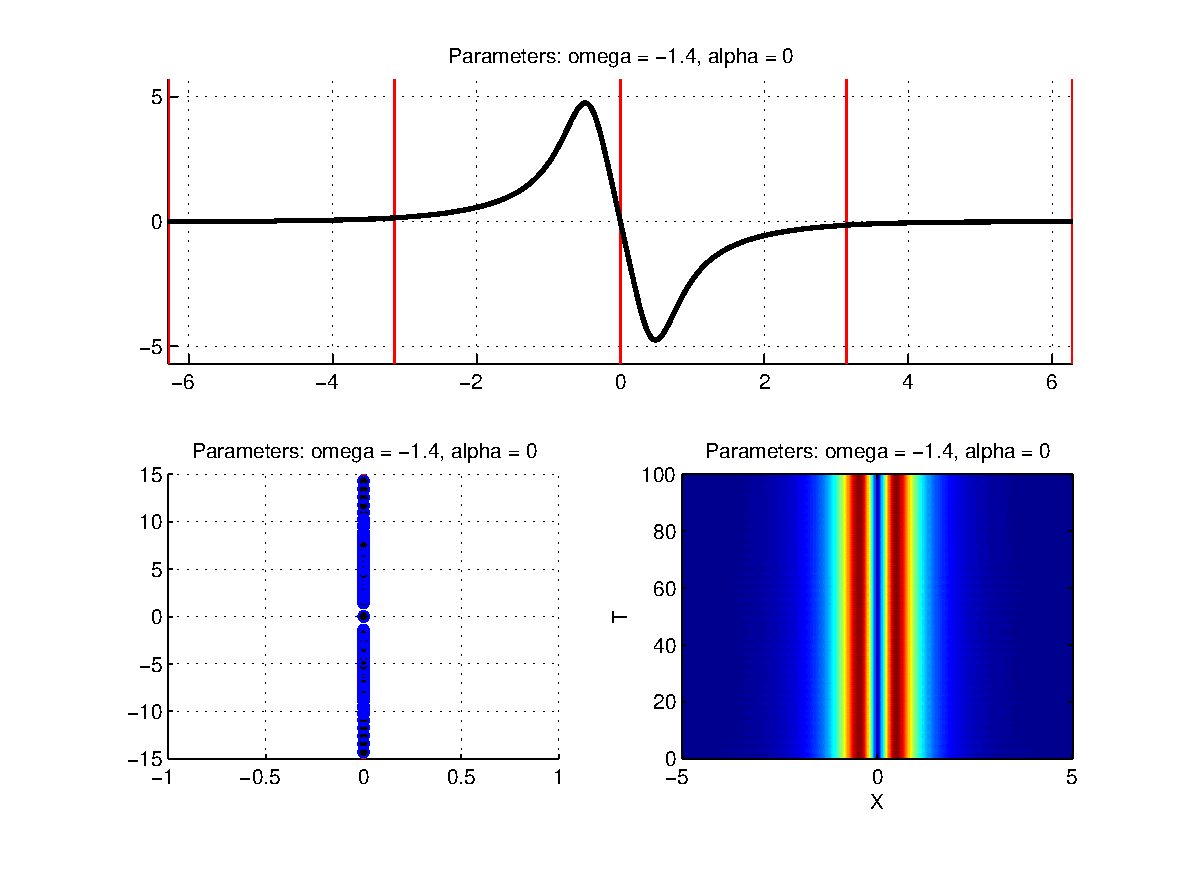
\includegraphics[width=1\linewidth]{pic/omega=-14alpha=0.eps} \ (B) $\omega = -1.4$}
	\end{minipage}}
\caption{Эволюция устойчивых дипольных солитонов и соответствующие им спектры при $\alpha = 0$.}
\label{pic:evolution_st}
\end{figure}
%
\begin{figure}
\center{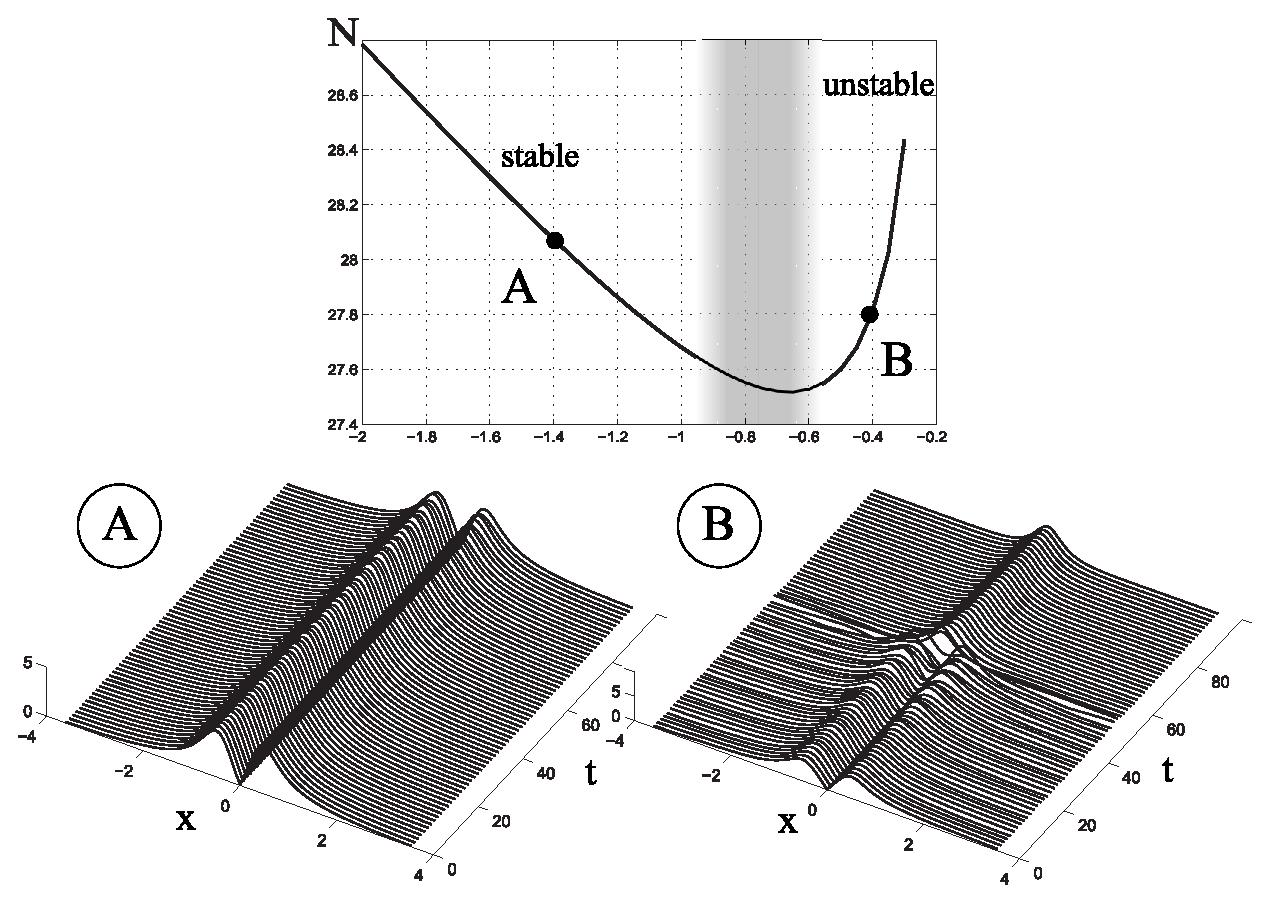
\includegraphics[width=0.8\textwidth]{pic/summary.eps}}
\caption{Численно построенная зависимость $N(\omega)$ при $\alpha = 0$; (A) устойчивый дипольный солитон, $\omega = -1.4$; (B) неустойчивый дипольный солитон, $\omega = -0.4$, в ходе эволюции превращается в устойчивый фундаментальный солитон с параметрами $\omega \approx -13.96$ и амплитудой $\approx 5.43$.}
\label{pic:summary}
\end{figure}
%